\chapter{一维情况}
首先,一个非常普适的框架就是如下的微分方程组
\begin{equation}
    \begin{aligned} 
        &\dot{x}_1 = f_1(x_1,\dots,x_n)  \\
        &\vdots \\
        &\dot{x}_1 = f_1(x_1,\dots,x_n)  
    \end{aligned} 
\end{equation}
其中 $ \dot{x_i} \equiv dx_i/dt $。
\par 举一个有阻尼的简谐振子,其运动方程为
\begin{equation}
    \begin{aligned} 
        m\frac{d^2x}{dt^2} + b\frac{dx}{dt} + kx = 0
    \end{aligned} 
\end{equation}
如果令 $ x_1 = x $ $ x_2 = \dot{x} $,则有 $ \dot{x}_1 = x_2 $,并且
\begin{equation}
    \begin{aligned} 
    \dot{x}_2 &= \ddot{x} = -\frac{b}{m}\dot{x} - \frac{k}{m}x\\
        &= -\frac{b}{m}x_2 - \frac{k}{m}x_1
    \end{aligned} 
\end{equation} 
这样子这个有阻尼的简谐振子方程就可以化为最开始比较普遍的形式
\begin{equation}
    \begin{aligned} 
    \dot{x}_1 &= x_2 \\
    \dot{x}_2 &= -\frac{b}{m} x_2 - \frac{k}{m}x_1
    \end{aligned} 
\end{equation}
这样的系统被称为线性的。因为等式右边只有一阶项。
\section{一维系统}
如果只有一个微分方程
\begin{equation}
    \begin{aligned} 
    \dot{x} = f(x)
    \end{aligned} 
\end{equation}
那么这样就是一维情况。(one dimensional or first-order systems)。
\par 首先来看一个例子来分析分析如何处理这样的系统。方程如下
\begin{equation}
    \begin{aligned} 
    \dot{x} = sin x
    \end{aligned} 
\end{equation}
这个方程是有解析解的。分离变量即可解得
\begin{equation}
    \begin{aligned} 
    t = -\ln |\csc x + \cot x| + C
    \end{aligned} 
\end{equation}
为了确定常数,假设$x(t=0) = x_0$。则解为
\begin{equation}
    \begin{aligned} 
    t = \ln \left| \frac{\csc x_0 + \cot x_0}{\csc x + \cot x}\right|
    \end{aligned} 
\end{equation}
我们可以根据下图来形象的理解x随时间的变化。我们想象液体沿着x轴流动,他的速度满足 $ \dot{x} = \sin x $ 。如图
所示: $ \dot{x} > 0 $ 时液体向右流动; $ \dot{x}  < 0$ 时液体向左流动; $ \dot{x} = 0 $时液体不
流动,这样的点就叫做 \textbf{fixed points}. 如果流汇聚,那么就是 \textbf{stable fixed points};如果
流往两边走则是 \textbf{unstable fixed points}。
\begin{figure}[htbp]
    \centering
    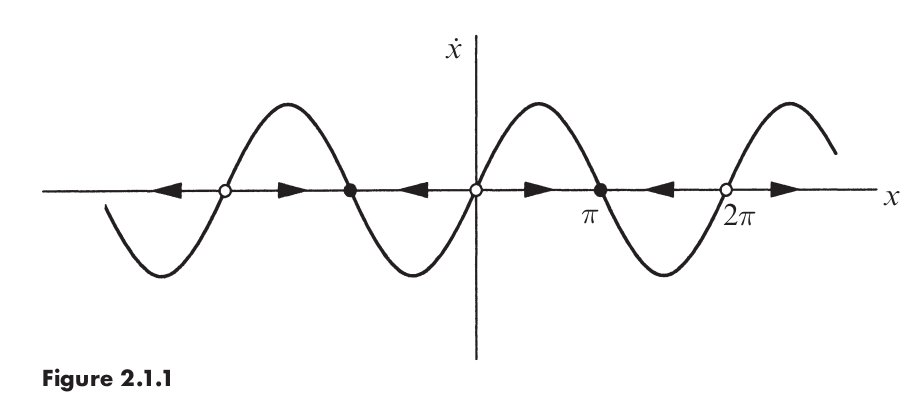
\includegraphics[width=0.8\textwidth]{figures/1-1.png}
    \caption{}
\end{figure}

\section{Fixed Points and Stablility}
和之前一样,我们想象一个液体沿着x轴流动,速率表达式为 $ f(x) $ 。这个想象的液体被称为 phase fluid, x轴被称为
phase space. $ f(x) > 0$时流向右, $f(x) < 0$时流向左。为了求解 $ \dot{x} = f(x) $ 我们放一个想象
的点(known as \textbf{phase point}) 在初始位置 $x_0$,然后观察这个点随流的移动。随着时间的推移,这个点
的轨迹是时间的函数,不妨设为 $x(t)$。这个方程称为初始位置为 $x_0$的轨迹(\textbf{trajectory}),也就是
微分方程的解嘛。
\begin{figure}[htbp]
    \centering
    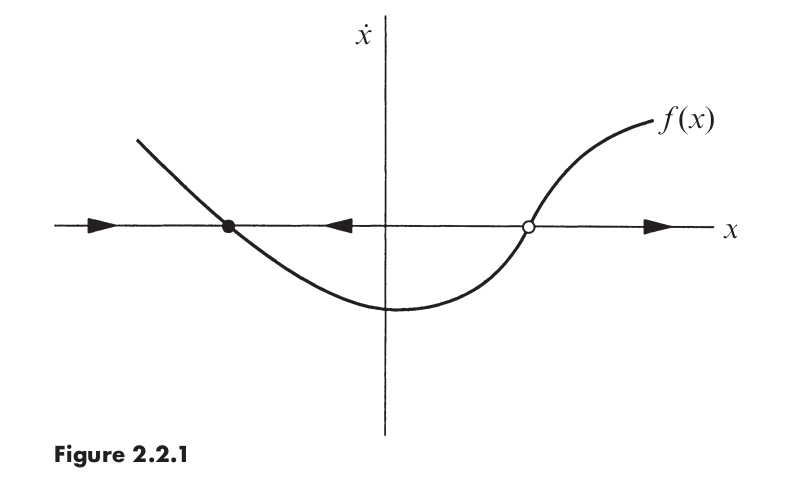
\includegraphics[width=0.8\textwidth]{figures/1-2.png}
    \caption{}
\end{figure}
而像上图用来定性描述这个系统的图,称为 \textbf{phas portratit}。
\par fixed points 代表了平衡解(equilibrium solutions)。 An equilibrium is defined to be stable if 
all sufficiently small disturbances away from it damp out in time. Thus stable equilibria 
are represented geometrically by stable fixed points. Conversely, unstable equilibria,
in which disturbances grow in time, are represented by unsatable fixed points.

\section{Potentials}
还有另外一种方式来理解 first-order system $ \dot{x} = f(x) $,这种方式基于物理中势的概念。我们
描述一个粒子沿着势垒壁向下滑,the \textbf{potential} $ V(x) $ 定义为
\begin{equation}
    \begin{aligned} 
    f(x) = - \frac{dV}{dx}
    \end{aligned} 
\end{equation}
利用链式求导法则并联立 $\dot{x} = f(x)$,有
\begin{equation}
    \begin{aligned} 
    \frac{dV}{dt} &= \frac{dV}{dx}\frac{dx}{dt} \\
                    &= -\left( \frac{dV}{dx}\right)^2 \le 0
    \end{aligned} 
\end{equation}
\section{Bifurcations}
The qualitative structure of the flow can changes as parameters are varied. In particular, 
fixed points can be created or destroyed, or their stability can change. These qualitative 
changes in the dynamics are called \textbf{bifurcations}, and the parameter values at which 
they occur are called \textbf{bifurcations points}.
\subsection{Pitchfork Bifurcations}
\subsubsection*{Supercritical Pitchfork Bifurcation}
The normal form of the supercritical pitchfork bifurcation is 
\begin{equation}
    \begin{aligned} 
    \dot{x} = rx - x^3
    \end{aligned} 
    \label{Bifurcation-1}
\end{equation}
Note that this equation is \textbf{invariant} under the change of variables $ x \rightarrow -x $.
That is,if we replace $ x $ by $ -x $ and then cancel the resulting minus signs on both sides 
of the equation and we get \ref{Bifurcation-1} back.
\begin{figure}[htbp]
    \centering
    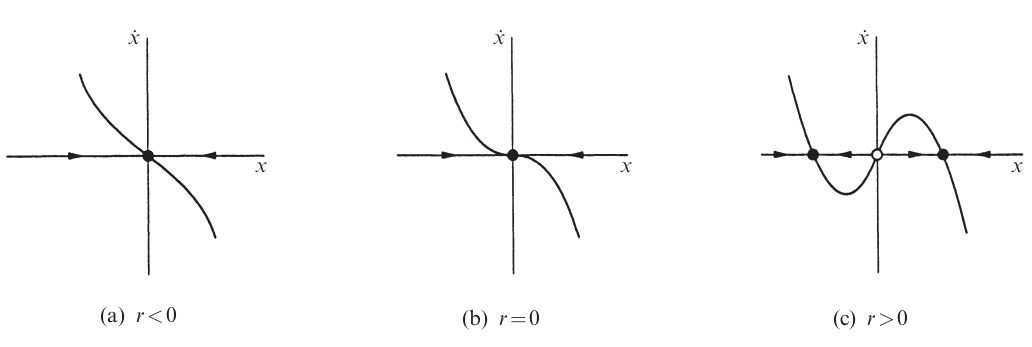
\includegraphics[width=0.8\textwidth]{figures/Bifurcation-1.png}
    \caption{the vector field for different values of r}
\end{figure}
当 $ r < 0 $ 时,原点是唯一的 fixed point,并且根据两边的流判断,它是 stable fixed point。当
 $ r = 0 $ 时,原点仍然是一个 stable fixed point。 但此时 $f'(x)|_{x=1} = 0$。 Now solutions 
 no longer decay exponentially fast --- instead the decay is a much slower algebraic function
 of time. This lethargic decay is called \textbf{critical slowing down} in the physics literature.
最后,当 $ r > 0 $ 时,原点变成了一个 unsatable fixed point. 而在原点两边新生成了两个对称的
stable fixed points,位置在 $ x^* - \pm \sqrt{r} $. 
\par 这个bifurcation 为什么叫做 pitchfork bifurcation? 我们可以画一个 bifurcation diagram.如下
\begin{figure}[htbp]
    \centering
    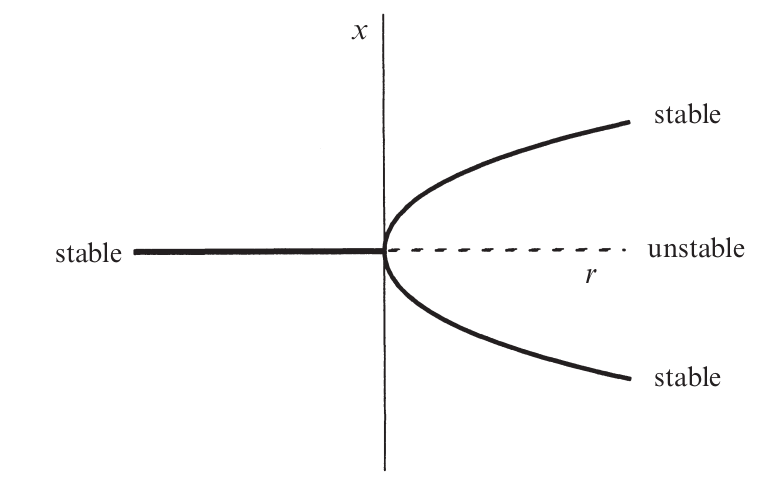
\includegraphics[width=0.8\textwidth]{figures/Bifurcation-2.png}
    \caption{}
    \label{Bifurcation-f1}
\end{figure}
可以看到,这个图的形状就像一个草叉!
\subsection*{Subcritical Pitchfork Bifurcation}
In the supercritical case $ \dot{x} = rx - x^3 $ discussed above, the cubic term is \textit{stabilizing}:
is acts as a restoring force that pulls $ x(t) $ back toward $ x = 0 $ . If instead the cubic 
term were \textit{destabilizing},as in 
\begin{equation}
    \begin{aligned} 
    \dot{x} = rx + x^3
    \end{aligned} 
\end{equation}
then we'd have a \textbf{Subcritical} pitchfork bifurcation.
\begin{figure}[htbp]
    \centering
    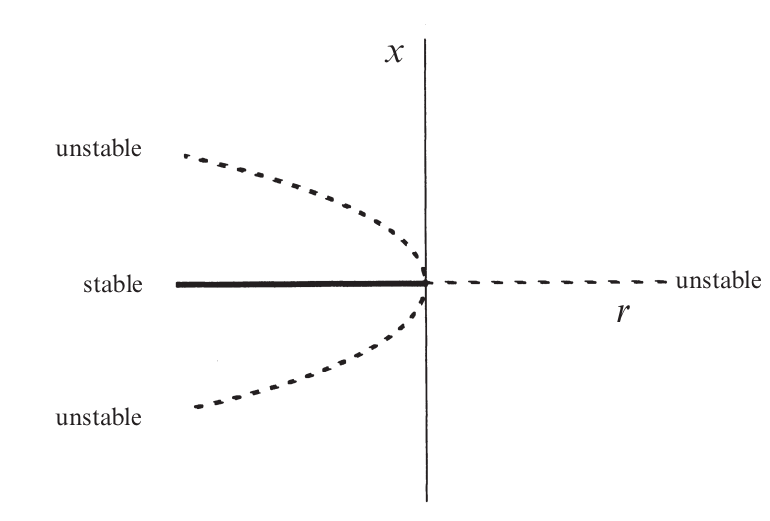
\includegraphics[width=0.8\textwidth]{figures/Bifurcation-3.png}
    \caption{}
\end{figure}
Compared to Figure (\ref{Bifurcation-f1}), the pitchfork is inverted. the nonzero fixed points 
$ x^* = \pm \sqrt{-r} $  are \textit{unstable}, and exist only \textit{below} the bifurcation $ (r<0) $, 
which motivates the term "subcritical."
\section{}